\documentclass[9pt]{beamer}
\mode<presentation>{}
\usepackage{beamerthemesplit} 

\setbeamertemplate{footline}[frame number]
\setbeamertemplate{headline}{}

\usepackage[english]{babel}
\usepackage[utf8x]{inputenc}
\usepackage{xcolor}
\usepackage{makecell}
\usepackage{listings}

\lstset{
   basicstyle=\fontsize{8}{8}\selectfont\ttfamily
}

\title[PPT - ROS Intro]{Introduction to ROS with Python}
\author{Evan Krell}
\institute{Texas A\&M University - Corpus Christi}
\date{November 2018}

\begin{document}

\begin{frame}
  \titlepage
\end{frame}

\begin{frame}{Outline}
  \tableofcontents
\end{frame}

\begin{section}{Introduction}
    \begin{frame}{Introduction}
        \begin{block}{Sources}
            \begin{columns}
                \begin{column}{0.5\textwidth}
                    \begin{center}
                        
\includegraphics[width=0.75\textwidth,trim={0cm 0cm 0cm 0cm},clip]{img/cover_agitr.jpg} \\
                        \textbf{Jason M. O'Kane} \\
                        \url{cse.sc.edu/~jokane/agitr}
                    \end{center}    
                \end{column}
                \begin{column}{0.5\textwidth}
                    \begin{center}
                        \textit{Structure Python-based ROS Package} \\
                        \textbf{Simon Birrel} \\
                        \url{artificialhumancompanions.com}
                        %
\includegraphics[width=\textwidth,trim={0cm 0cm 0cm 0cm},clip]{img/cover_agitr.jpg}
                    \end{center}
                \end{column}    
            \end{columns}
        \end{block}
    \end{frame}
    \begin{frame}{Introduction}
        \begin{block}{Package for this Tutorial}
            The content presented is demonstrated in an ROS package written in Python.
        \end{block}
        \begin{block}{Location}
            \url{https://github.com/ekrell/ros_python_workshop}
        \end{block}
        \begin{block}{Turtlesim Environment}
            % \begin{center}
                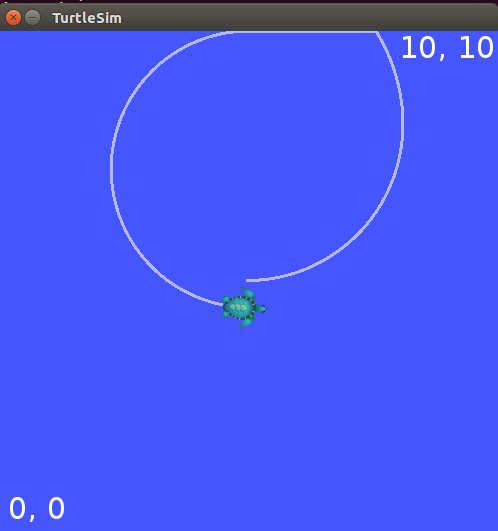
\includegraphics[width=0.4\textwidth,trim={0cm 0cm 0cm 0cm},clip]{img/turtlesim.png}
            % \end{center}
        \end{block}
    \end{frame}
\end{section}



\begin{section}{Getting Started}
    \begin{frame}{Getting Started} \label{frame:packages}
        \begin{block}{Packages}
            \begin{center}
                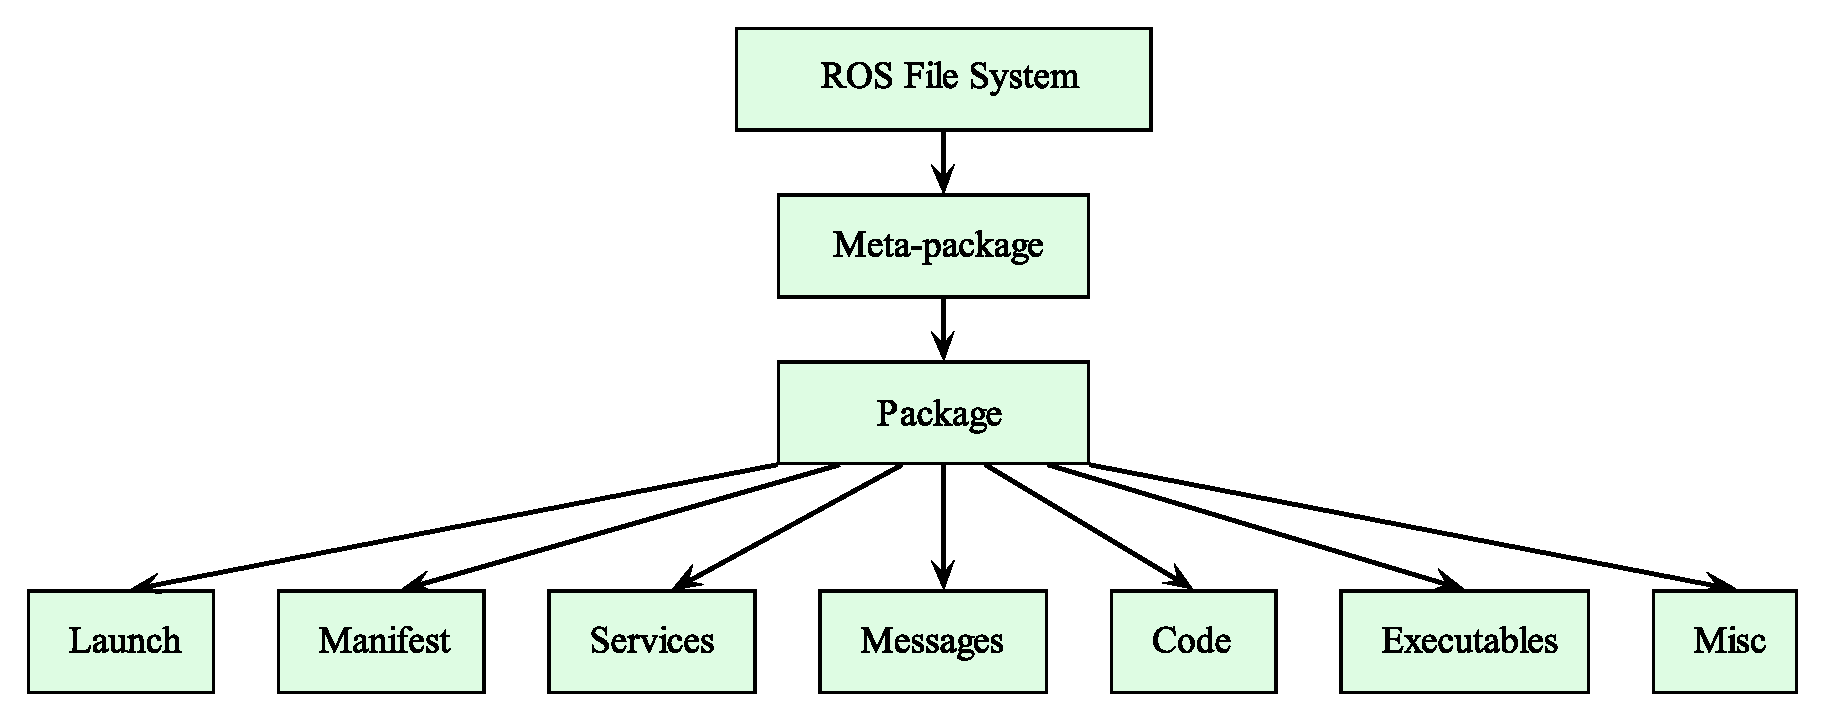
\includegraphics[width=\textwidth,trim={0cm 0cm 0cm 0cm},clip]{img/ros_packages.eps}
            \end{center}        
        \end{block}
    \end{frame}
    \begin{frame}{Getting Started}
        \begin{columns}
            \begin{column}{0.5\textwidth}
                \begin{block}{Packages}
                    \begin{itemize}
                        \item Collection of files that fulfill single purpose (code, executables, etc)
                        \item Simply a directory with \textbf{manifest} file called \texttt{package.xml}
                        \item \textbf{Manifest} file has package definition, with name, version, dependencies
                        \item Facilitates organization, sharing
                    \end{itemize}
                \end{block}
            \end{column}
            \begin{column}{0.5\textwidth}
                \begin{center}
                    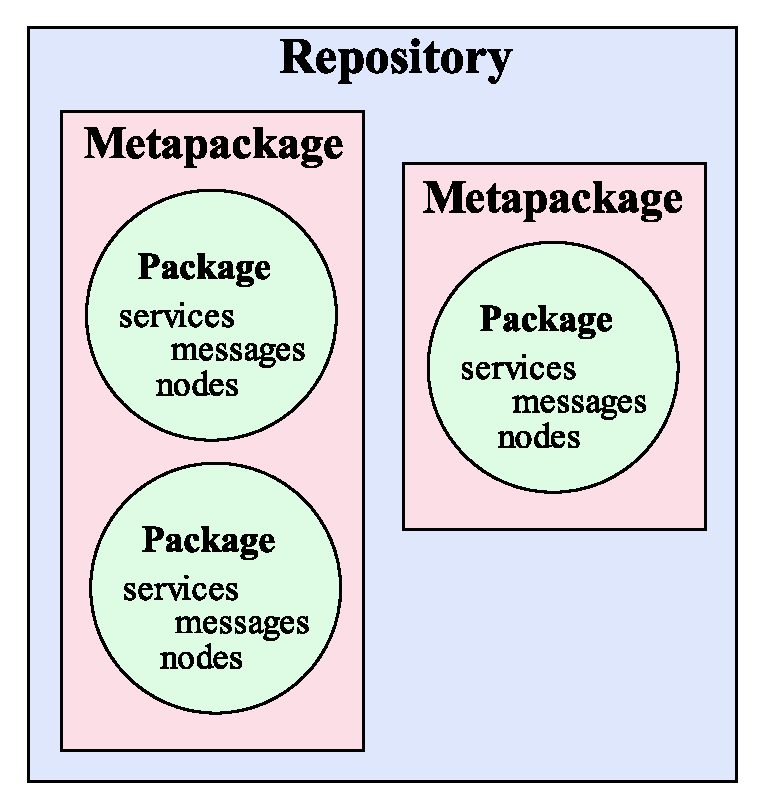
\includegraphics[width=\textwidth,trim={0cm 0cm 0cm 0cm},clip]{img/ros_repos.eps}
                \end{center}           
            \end{column}        
        \end{columns}
    \end{frame}
    \begin{frame}{Getting Started} \label{frame:master}
        \begin{columns}
            \begin{column}{0.5\textwidth}
                \begin{block}{ROS Master}
                    \begin{itemize}
                        \item Maintains directory of nodes, messages, services, parameters, etc
                        \item Enables communication among nodes
                        \item \textbf{Parameter server}: directory of parameters and values
                    \end{itemize}
                \end{block}
            \end{column}
            \begin{column}{0.5\textwidth}
                \begin{center}
                    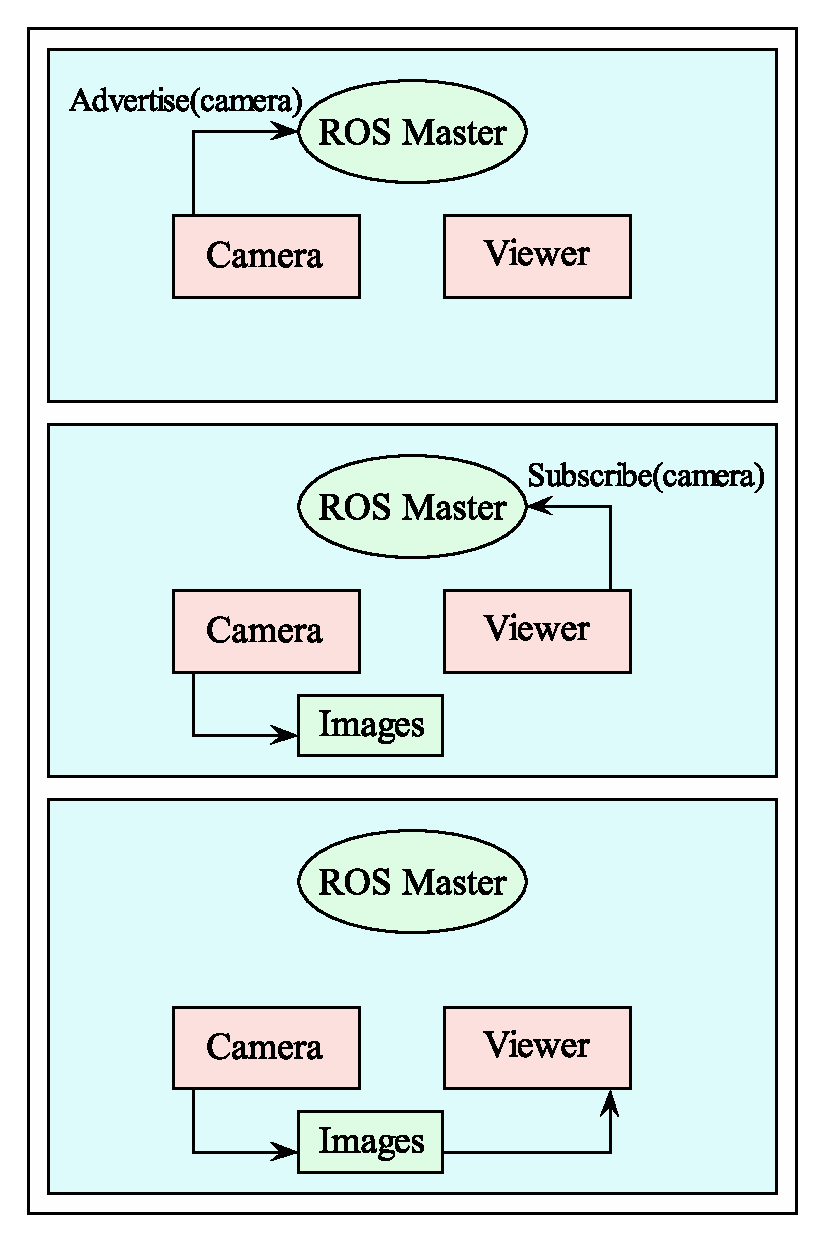
\includegraphics[width=0.95\textwidth,trim={0cm 0cm 0cm 0cm},clip]{img/ros_master.eps}
                \end{center}           
            \end{column}        
        \end{columns}
    \end{frame}
    \begin{frame}{Getting Started} \label{frame:node}
        \begin{columns}
            \begin{column}{0.5\textwidth}
                \begin{block}{Nodes}
                    \begin{itemize}
                        \item Single executable using ROS
                        \item Communicate over \textbf{topics} (publish, subscribe)
                    \end{itemize} 
                \end{block}
            \end{column}
            \begin{column}{0.5\textwidth}
                 \begin{center}
                    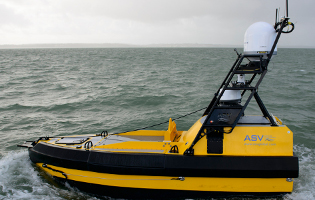
\includegraphics[width=0.85\textwidth,trim={0cm 0cm 0cm 0cm},clip]{img/ASV-C-Worker-USV.jpg}
                \end{center}            
            \end{column}    
        \end{columns}
        \begin{center}
            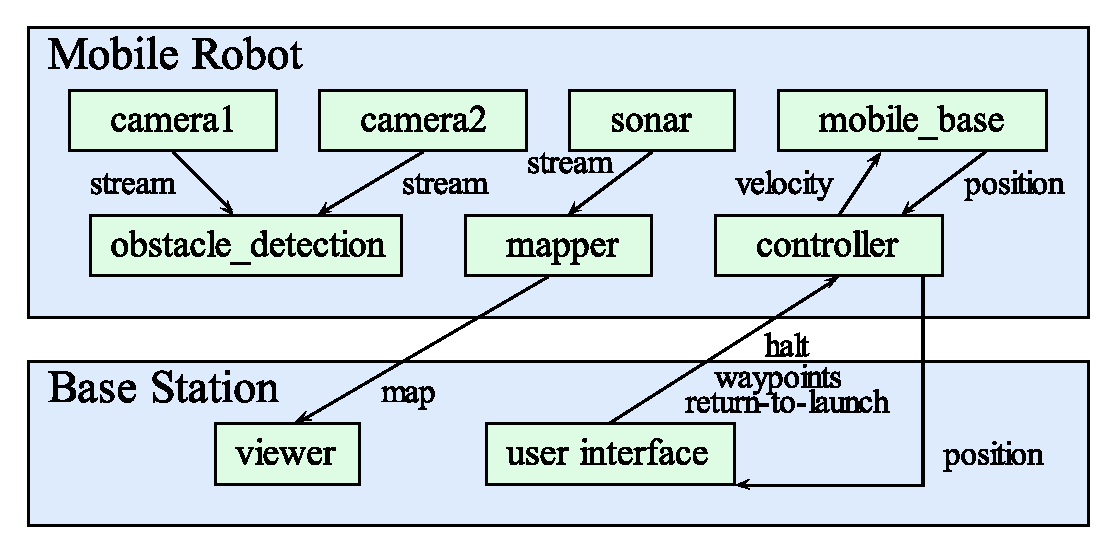
\includegraphics[width=0.9\textwidth,trim={0cm 0cm 0cm 0cm},clip]{img/ros_nodes.eps}
        \end{center}                      
    \end{frame}
    \begin{frame}{Getting Started} \label{frame:topics_messages}
        \begin{block}{Topics}
            \begin{itemize}
                \item Named buses for node communication
                \item Each has a specific message \textbf{type}
                \item Types are integers, floats, strings, and composite structures
            \end{itemize} 
        \end{block}
        \begin{block}{Messages}
            \begin{itemize}
                \item Units of communication
                \item Each message is of a specific \textbf{type}
            \end{itemize} 
        \end{block}
            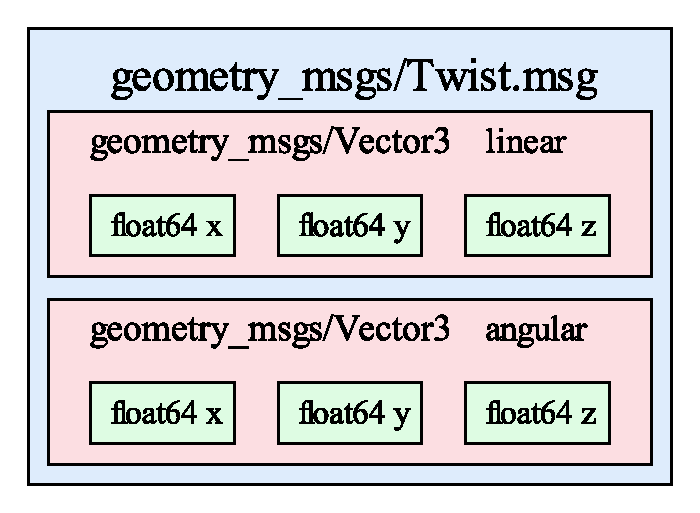
\includegraphics[width=0.45\textwidth,trim={0cm 0cm 0cm 0cm},clip]{img/ros_message.eps}
    \end{frame}
\end{section}

\begin{section}{Writing ROS Programs}
    \begin{frame}{Writing ROS Programs}
        \begin{block}{Install ROS}
            Installation guide:
            \url{wiki.ros.org/ROS/Installation}
        \end{block}   
        \begin{block}{Setup Catkin}
            \textbf{catkin}: build system for ROS
            \url{/wiki.ros.org/catkin}
        \end{block}           
        \begin{block}{ROS for Python}
            \textbf{rospy}: ROS Python library
            \url{wiki.ros.org/rospy/Tutorials}
        \end{block}
    \end{frame}
    \begin{frame}{Writing ROS Programs}
        \begin{block}{Install ROS Package}
            \begin{itemize}
                \item[] \lstinline{cd ~/catkin_ws/src}
                \item[] \lstinline{git clone https://github.com/ekrell/ros_python_workshop.git}
                \item[] \lstinline{cd ~/catkin_ws}
                \item[] \lstinline{catkin_make}
            \end{itemize}
        \end{block}
        \begin{block}{Execute ROS package}
            \begin{itemize}
                \item[] \lstinline{roscore}
                \item[] \lstinline{rosrun PACKAGE_NAME SCRIPT.py}
            \end{itemize}
        \end{block}
    \end{frame}
\end{section}

\begin{section}{Log Messages}
    \begin{frame}{Log Messages}
        \begin{block}{ROS Logging}
        \begin{itemize}
            \item[] View log in console: \lstinline{rostopic echo /rosout}
            \item[] View log in GUI: \lstinline{rqt_console}
        \end{itemize}
        \end{block}
        \begin{block}{Log Message Severity}
            \begin{columns}
                \begin{column}{0.7\textwidth}
                    \begin{itemize}
                        \item[] \textbf{Debug:} \lstinline{rospy.logdebug(msg, *args)}
                        \item[] \textbf{Warn:} \lstinline{rospy.logwarn(msg, *args)}
                        \item[] \textbf{Info:} \lstinline{rospy.loginfo(msg, *args)}
                        \item[] \textbf{Error:} \lstinline{rospy.logerr(msg, *args)}
                        \item[] \textbf{Fatal:} \lstinline{rospy.logfatal(msg, *args)}
                    \end{itemize}
                \end{column}
                \begin{column}{0.3\textwidth}
                    \begin{itemize}
                    \item[] Lowest severity
                    \item[] \hfill 
                    \item[] \textbf{...}
                    \item[] \hfill 
                    \item[] Highest severity
                    \end{itemize}
                \end{column}
            \end{columns}
        \end{block}
    \end{frame}
    \begin{frame}[fragile]{Log Messages}
        \begin{block}{Python Example}
            \begin{verbatim}
rospy.loginfo_throttle(10, status2str(pose, params["goal"]))
            \end{verbatim}
        \end{block}
        \begin{block}{Result}
        \lstinline{rostopic echo /rosout}
            \begin{lstlisting}[language=Python]
    level: 2
    name: "/purepursuit"
    msg: "Position: (x:5.5, y:5.5, theta:0.0), Goal: (x:9, y:9)"
            \end{lstlisting}
        \end{block}
    \end{frame}
\end{section}





\begin{section}{Graph Resources}
    \begin{frame}{Graph Resources}
        \begin{block}{Naming Scheme}
            \begin{itemize}
                \item ROS organizes nodes, topics, services, parameters in graph
                \item Thus, elements are called graph resources
                \item Flexible naming scheme for referencing these resources
                \item Facilitates modularity and existence of duplicate executions of same node
                \item But can be difficult to find where resources come from at first
            \end{itemize}
             \begin{center}
                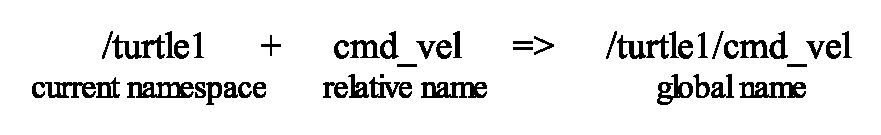
\includegraphics[width=0.85\textwidth,trim={0cm 0cm 0cm 0cm},clip]{img/ros_names.eps}
            \end{center}
        \end{block}
    \end{frame}
\end{section}

\begin{section}{Launch Files}
    \begin{frame}[fragile]{Launch Files}
        \begin{block}{Launch Multiple Nodes}
            \begin{itemize}
                \item Launch files setup and run multiple nodes
                \item Relieves burden of opening multiple terminals, executing each node in order, remembering all parameters, etc
                \item \textbf{Modular:} launch files can call launch files
                \item \lstinline{roslaunch ros_python_workshop ros_python_workshop}
                \item \textbf{Ctrl-C} will (ideally) gracefully shut down each node
            \end{itemize}
        \end{block}
        \begin{block}{Example}
            \lstinline{ros_python_workshop/launch/ros_python_workshop.launch} \\
            \lstinline{rosnode list}
            \begin{lstlisting}[language=Python]
    /purepursuit
    /rosout
    /turtlesim_node
            \end{lstlisting}
        \end{block}
    \end{frame}
\end{section}

\begin{section}{Parameters}
    \begin{frame}{Parameters}
        \begin{block}{Parameter Server}
            \begin{itemize}
                \item Handled within ROS Master
                \item Dictionary shared by nodes
                \item Setting \& getting inside and outside node
                \item Just \textbf{strings}, not ROS message types
                \item \textbf{Caution:} Node must manually check for param changes
            \end{itemize}
        \end{block}
        \begin{block}{Console Basics}
            \begin{itemize}
                \item[] \lstinline{rosparam list}
                \item[] \lstinline{rosparam get goal}
                \item[] \lstinline{rosparam get roslaunch}
                \item[] \lstinline{rosparam set goal "[9, 9]"}
                \item[] \lstinline{rosparam dump testdump.txt roslaunch}
                \item[] \lstinline{rosparam load testdump.txt roslaunch}
            \end{itemize}
        \end{block}        
    \end{frame}
\end{section}

\begin{section}{Services}
    \begin{frame}{Services}
        \begin{block}{Services}
            Publishing and subscribing to topics are not the only way to handle messages in ROS. 
            Services are similar to the message passing you may be familiar with in MPI. Content of messages specified by \textit{service data type}. 
        \end{block}
        \begin{itemize}
            \item Service calls are bi-directional: a sender expects a response
            \begin{itemize}
                \item With topics: you just send messages. No idea if any nodes are subscribed
                \item With services: send to a specific node and wait for response
            \end{itemize}
            \item Service calls are one-to-one: 
                \item With topics: arbitrary number of opt-in recipients. 
                \item With services: 
                \begin{itemize}
                    \item A sends \textit{request} to B: A $\rightarrow$ B
                    \item B sends \textit{respond} to A: A $\leftarrow$ B
                \end{itemize}
        \end{itemize}
        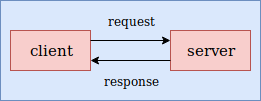
\includegraphics[width=0.45\textwidth,trim={0cm 0cm 0cm 0cm},clip]{img/services.png}
    \end{frame}
    
    \begin{frame}[fragile]{Services}
        \begin{block}{Command Line Service Management}
            \begin{itemize}
                \item[] List all services: \lstinline{rosparam list}
                    \begin{lstlisting}
    /clear
    /kill
    /reset
    /rosout/get_loggers
    /rosout/set_logger_level
    /spawn
    /turtle1/set_pen
    /turtle1/teleport_absolute
    /turtle1/teleport_relative
    /turtlesim/get_loggers
    /turtlesim/set_logger_level
                    \end{lstlisting}
                \item[] List all node-specific services: \lstinline{rosnode info turtlesim}
                    \begin{lstlisting}
    /turtle1/teleport_absolute
    /turtlesim/get_loggers
    /turtlesim/set_logger_level
    /reset
    /spawn
    /clear
                    \end{lstlisting}                
                \end{itemize}
            \end{block}
    \end{frame}
    \begin{frame}[fragile]{Services}
        \begin{block}{Command Line Service Management}   
                \begin{itemize}
                    \item[] Find a service's host node: \lstinline{rosservice node /spawn}
                    \begin{lstlisting}
    /turtlesim
                    \end{lstlisting}
                \item[] Find a service's data type: \lstinline{rosservice into /spawn} \\
                    \begin{lstlisting}
    Node: /turtlesim
    URI: <your URI>
    Type: turtlesim/Spawn
    Args: x y theta name
                    \end{lstlisting}
                \item[] Inspect a service's data type: \lstinline{rossrv show turtlesim/Spawn}
                    \begin{lstlisting}
float32 x
float32 y
float32 theta
string name
---
string name
                    \end{lstlisting}
                \item[] Call a service: \lstinline{rosservice call /spawn 5 5 0 Sally} \\
                Adds turtle named Sally at with position (x:5, y:5, theta:0) \\
                The \textit{/spawn} service was used within the turtlesim code.
            \end{itemize}
        \end{block}     
    \end{frame}
\end{section}

\begin{section}{Recording \& Replaying Messages}
    \begin{frame}{Recording \& Replaying Messages}
        \begin{block}{Message-based Architecture}
            \begin{itemize}
                \item Core to ROS: nodes act upon information on topics \& services
                \item Nodes should not care \textit{who} sends that information
                \item Example: turtlebot should not know if move commands come from command line, keyboard, or joystick 
            \end{itemize}
        \end{block}
        \begin{block}{rosbag}
            \begin{itemize}
                \item rosbag allows you to record messages and replay them
                \item Start recording: \\
                \lstinline{rosbag record -O filename.bag topic-names} \\
                All messages published on the topic-names will be recorded to file filename.bag
                \item Replay recording: \\
                \lstinline{rosbag play filename.bag} \\
                Those messages will be republished on their original topics. \\
                Original timing is preserved!
            \end{itemize}
        \end{block}
    \end{frame}
    \begin{frame}[fragile]{Recording \& Replaying Messages}
        \begin{block}{Bags in Launch Files}
            \begin{itemize}
                \item A launch file \textit{record} node
                    \begin{lstlisting}
    <node
    pkg="rosbag"
    name="record"
    type="record"
    args="-O filename.bag topic-names"
    />
                    \end{lstlisting}                
                \item Launch file \textit{play} node
                    \begin{lstlisting}
    <node
    pkg="rosbag"
    name="play"
    type="play"
    args="filename.bag"
    />
                    \end{lstlisting}
            \end{itemize}
        \end{block}
    \end{frame}
    
    
\end{section}

\begin{section}{References}
    \begin{frame}{Image Sources}
        \begin{itemize}
            \item [Slide \ref{frame:packages}] Mastering ROS for Robotics Programming
            \item [Slide \ref{frame:master}] \url{wiki.ros.org/Master}
            \item [Slide \ref{frame:node}] ASV C-Worker USV 
        \end{itemize}
    \end{frame}
\end{section}
\end{document}
